\chapter{GitLab}

\section{General Information}
GitLab is a web-based DevOps lifecycle tool that provides a Git-repository manager offering wiki, issue-tracking, and continuous integration/continuous deployment (CI/CD) pipeline features, using an open-source license.
GitLab was developed by GitLab Inc. and it's available in multiple editions, namely:
\begin{itemize}
    \item GitLab Community Edition (CE)
    \item Enterprise Edition (EE)
    \item GitLab.com hosted service.
\end{itemize}
Each edition has a variety of features designed to meet different needs. (\cite{refAboutGitLab})

\section{Self-hosting}
GitLab provides self-hosted options, which allows users to host the platform on their own servers.
This option is particularly useful for organizations that want to keep their codebase and data in-house for privacy or security reasons.
GitLab can be installed on various systems with the aid of Omnibus, a versatile package provided by GitLab.
Omnibus simplifies the installation process by bundling all necessary dependencies, and it provides an easy method to manage and update the GitLab instance.

\section{Adding CI Functionality with Self Hosted Agents}
GitLab has built-in CI/CD, which means there's no need for an external tool.
Users can configure the CI/CD pipelines through a 'gitlab-ci.yml' file in the root of their repository.
When changes are pushed to the repository, GitLab will automatically execute the tasks defined in this file.

In a self-hosted environment, these tasks are run on what are known as 'Runners'.
Runners are agents or servers that are configured to execute the code defined in your .yml file.

\begin{figure}[H]
	\centering
	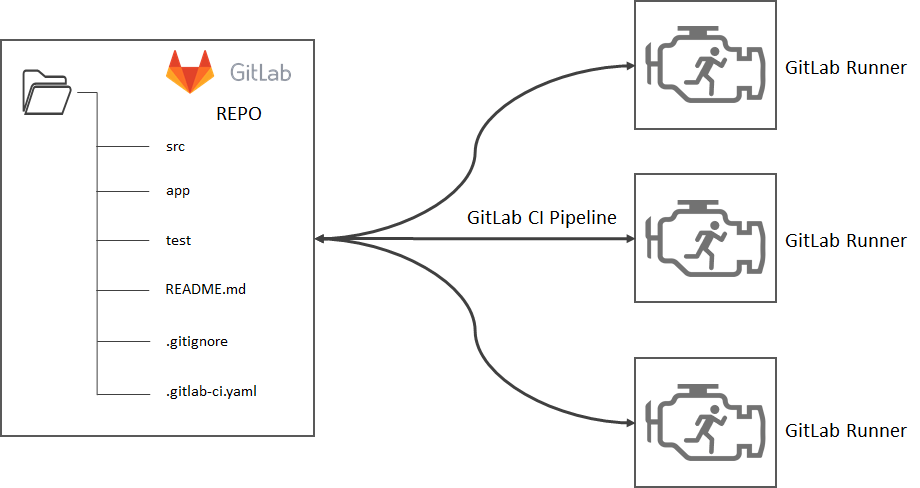
\includegraphics[width=14cm]{images/gitlab_runners.png}
	\caption{How GitLab Runners work (\cite{refGitLabRunners})}
	\label{fig:gitlab_runners}
\end{figure}

These Runners can also be self-hosted, meaning that not only is your codebase internal, but also the environments where your pipelines are run, increasing security and potentially reducing costs.
Configuring self-hosted Runners involves installing the Runner software on a suitable server, registering it with your GitLab instance, and then specifying that Runner in your 'gitlab-ci.yml' file.

\section{Usage in the assignment}

During walking through the documentation of GitLab we realized very quickly, the most efficient way to set up GitLab is to run a container from the official GitLab container image. For the container runtime we chose Docker. As base operating system we chose Debian, Ubuntu would have been our second choice. Docker does not integrate very well with RHEL based systems as those prefer Podman.\\

For our example we defined to have exactly on GitLab Runner, also Debian based with Docker runtime. The goal is to let the Runner build everything inside containers, so not additional software installation is required (beside the Runner itself).
